%\include{macro_lecture}
\section*{Cíl laboratorního cvičení}
\begin{itemize}
  \item seznámit se s nástroji pro správu sítě
  \item seznámit se s formátem Cisco Netflow pro ukládání statistických dat a nástrojem pro čtení NetFlow {\bf nfdump}
  \item naučit se pracovat s protokolem Syslog a nástrojem {\bf rsyslog}
  \item konfiguraci nástrojů pro monitoring {\bf Icinga2}
\end{itemize}

\section*{Pokyny}
\begin{itemize}
  \item Do zadání nepište, slouží pro další skupiny. PDF verzi zadání
  i šablony konfiguračních souborů lze najít v IS u předmětu ISA.
  
  \item Na konci laboratorního cvičení nezapomeňte na poslední bod,
  tj. na {\bf Ukončení práce v laboratoři}!
  
  \item Zapněte si počítače pod Linux a přihlaste se jako uživatel {\bf user} s heslem {\bf user4lab}
  
  \item Smažte pravidla ve firewallu příkazem {\tt iptables --flush}
  
  \item Volitelně můžete použít k přístupu na virt. počítače SSH (adresy 192.168.56.10, 192.168.56.20)
\end{itemize}

\newpage
%\section{Laboratorní úlohy}

%NETFLOW
\section{NetFlow}
\begin{itemize}
	\item Úkol:
	\begin{itemize}
		\item Seznámit se možnostmi měření provozu pomocí NetFlow. NetFlow slouží pro
		přenos statistik o jednotlivých tocích dat vznikajících při komunikaci po síti.
		Záznamy NetFlow, s~nimiž budete během cvičení pracovat, jsou
		pořízeny ze sítě VUT a~anonymizovány. V~druhé části úkolu
		budete pracovat s~daty pořízenými sondou FlowMon.
	\end{itemize}
	\item Příkazy:
	\begin{itemize}
		\item {\tt nfdump}
	\end{itemize}
	\item Postup:
	\begin{enumerate}
		\item Na Vašem počítači se v adresáři {\tt /home/user/isa5/netflow} nachází
		anonymizovaná kolekce NetFlow dat. Tento adresář bude vstupem programu
		{\tt
nfdump}, který využijte ke kladení dotazů nad NetFlow daty.
		\item Prostudujte manuálovou stránku nástroje {\tt nfdump}.
		\item Dotažte se na TOP 20 IP adres podle počtu přenesených bajtů. 
		\begin{itemize}
			\item V manuálové stránce si najděte, co dělají přepínače {\tt -R, -s, -n, -O}.
			\item Nezapomeňte, že zpracovávaná data jsou relativně objemná. Dosažení výsledku tedy chvíli potrvá.
		\end{itemize}
		\item Zjistěte, jak velké datové přenosy připadají na jednotlivé protokoly. (Statistika protokolů)
		\begin{itemize}
			\item Všimněte si rozdílů v podílech podle toků a podle přenesených bajtů.
		\end{itemize}
		\item Vyfiltrujte si toky se zdrojovou IP 162.35.0.190. Zaměřte se na čísla portů.
		Je aktivita zdroje něčím podezřelá?
		
		\item {\bf Výstupy NFdump předveďte cvičícímu}.
	\end{enumerate}
\end{itemize}

%SYSLOG
\section{Syslog}
  \begin{itemize}
    \item Úkol: 
    \begin{itemize}
      \item Seznámit se s protokolem Syslog, který slouží pro přenos
      logovacích zpráv ze spravovaných zařízení. Pojmem Syslog je často označováno také
      programové vybavení implementující samotný přenos, třídění a ukládání zpráv na disk.
      \item Pracujte ve dvojicích, kde jeden bude v~roli serveru a~druhý v~roli klienta.
      \item Pro práci využijte nástroj {\tt rsyslogd}, který bude sloužit jako server i klient.
      K otestování využijte nástroj {\tt logger}.
      \item Na klientovi následně omezte přeposílání pouze na zprávy konkrétního typu.
      \item Na obou stanicích pracujte jako uživatel root.
    \end{itemize}
    \item Příkazy:
       \begin{itemize}
            \item {\tt rsyslogd(8)} -- démon pro Syslog.
            \item {\tt rsyslog.conf(5)} -- Popis konfigurace rsyslog démona.
            \item {\tt logger(1)} -- Nástroj pro generování Syslog zpráv.
        \end{itemize}
    \item Postup:
       \begin{enumerate}
            \item {\bf Na serveru} povolte naslouchání na síťovém soketu. Do souboru {\tt /etc/rsyslog.conf} přidejte nebo odkomentujte:
\begin{verbatim}
  $ModLoad imudp
  $UDPServerRun 514
\end{verbatim}

            \item {\bf Na klientovi} nakonfigurujte rsyslog démona tak, aby odesílal veškeré zprávy
         z klienta na serveru pomocí UDP. Jako oddělovač použijte výhradně tabulátor nikoliv mezery.
         Do souboru {\tt /etc/rsyslog.conf} přidejte následující pravidlo:
\begin{verbatim} 
 *.*<TAB>@<doménové_jméno_serveru>:<číslo_portu>
\end{verbatim}

            \item {\bf Na serveru i klientovi} restartujte Syslog démona: 
\begin{verbatim}
  systemctl restart rsyslog
\end{verbatim} 

            \item {\bf Z klienta} ověřte správnou konfiguraci vygenerováním testovací Syslog 
         zprávy pomocí nástroje {\tt logger}:
\begin{verbatim} 
  logger -d <obsah_zprávy>
\end{verbatim} 
        
            \item Zpráva byla přeposlána na server, kde ji lze najít na konci souboru
         {\tt /var/log/messages}.

\begin{verbatim} 
  tail -f /var/log/messages | grep <doménové_jméno_klienta>
\end{verbatim} 

            \item  Na klientovi pokračujte v generování Syslog zpráv a 
         na serveru sledujte příchozí Syslog zprávy pomocí {\tt wireshark}. Na jakém
         portu a jakým protokolem jsou Syslog zprávy zasílány.      

            \item Otevřete si manuálovou stránku {\tt rsyslog.conf} a zjistěte, jaké zařízení a priority
         zpráv Syslog poskytuje (kapitola {\bf SELECTORS}). 
\begin{verbatim} 
  man rsyslog.conf
\end{verbatim} 
        
         \item Ze znalosti zařízení a priorit nakonfigurujte klienta, aby posílal na server 
         zprávy související s autentizací na úrovni info, tj. upravte již existující pravidlo pro přeposílání
         veškerých zpráv na server v souboru {\tt /etc/rsyslog.conf}. Nezapomeňte restartovat Syslog démona. 
         
\begin{verbatim} 
  Syntax pravidel: <facility>.<priority><TAB><action>
\end{verbatim} 
         \item Pokuste se o neúspěšné ssh připojení na klienta a podívejte se ve wiresharku, jakou zprávu zaslal klient serveru. Následně odešlete z klienta zprávu příkazem {\tt logger}. Při správné konfiguraci by se tato zpráva neměla odeslat. {\bf Ukažte cvičícímu pakety s odeslanou autentizační zprávou}.

       \end{enumerate}
   \end{itemize}

%ICINGA2
\section{Icinga2}
  \begin{itemize}
    \item Úkol: 
    \begin{itemize}
      \item Seznámit se s nástrojem Icinga2 pro monitorováni zařízení a služeb.
      \item Na klientské stanici nakonfigurovat nakonfigurovat kontroly služeb a hostů.  
    \end{itemize}
    \item Poznámka:
        \begin{itemize}
	        \item Zapněte si VirtualBox (Applications $\rightarrow$ System Tools), kde se nacházejí 2 virtuální počítače, {\bf isa-icinga-master} a {\bf isa-icinga-provider}. Přepněte se do panelu se snapshoty pomocí Machine $\rightarrow$ Tools $\rightarrow$ Snapshots a~zkontrolujte zda jsou počítače v předdefinovaném stavu {\bf Clean} (obr. \ref{fig:revert}). Pokud ne, proveďte obnovení tlačítkem {\bf Restore} do tohoto stavu. Volbu {\bf Create snapshot of the current machine state} vypněte.
            
            \begin{figure}[!ht]
            	\caption{Uvedení virt. počítače do snapshotu Clean}
            	\centering
            	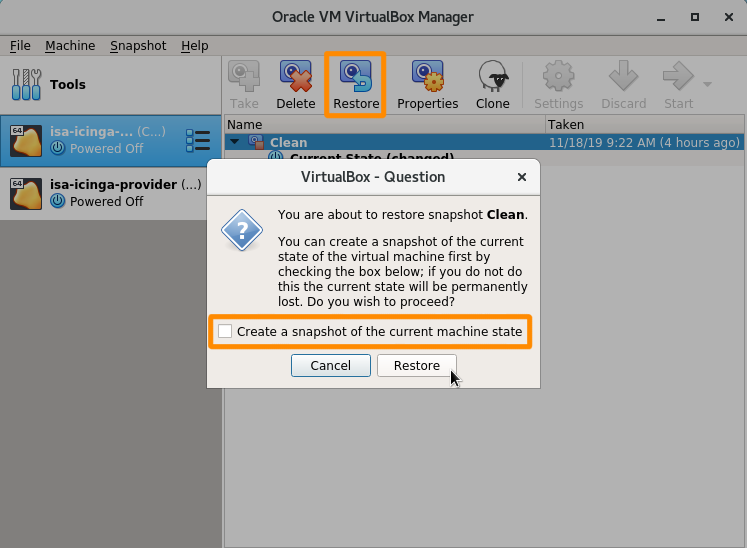
\includegraphics[width=0.67\linewidth]{files/vbox-revert.png}
            	\label{fig:revert}
            \end{figure}
            
            \item Všechny virtuální počítače mají root účet s údaji shodnými s laboratorním účtem
            \begin{itemize}
            	\item {\bf root/root4lab}
            \end{itemize}
        \end{itemize}
		\begin{figure}[!ht]
			\caption{Ilustrace zapojení virt. prostředí}
			\centering
	    	\includegraphics*[width=0.5\linewidth]{files/vbox-network.pdf}
		\end{figure}
    \item Postup:
       \begin{enumerate}
       		\item Spusťte virt. počítače isa-icinga-master a isa-icinga-provider. Příkazem ping ověřte, že
       		jsou tyto počítače dostupné.
            \item Otevřete si webový prohlížeč a zadejte adresu 
            {\it http://192.168.56.10/icingaweb2}. Dostanete se na webové rozhraní Icingy2,
            která běží na počítači {\bf isa-icinga-master}. Přihlaste se pod uživatelem {\bf isa} a heslem {\bf user4lab}.
            \item Na virt. počítači isa-icinga-master ve složce {\it /etc/icinga2/conf.d} najdete soubor {\bf hosts.conf}. Odkomentujte a doplňte potřebnou konfiguraci, aby systém Icinga2 
            monitoroval virt. počítač {\bf isa-icinga-provider} a~služby {\bf http} a~{\bf snmp-free-memory}. Pole {\tt host\_name}
            se musí shodovat s názvem Host objektu.
            
\begin{verbatim}
object Host "Provider" {
    address = "<IP ADDRESS>"
    check_command = "hostalive"
}

object Service "http" {
    max_check_attempts = 4
    check_interval = 10m
    retry_interval = 10m
    host_name = "<HOST NAME OF OBJECT>"
    check_command = "http"
}

object Service "snmp-free-memory" {
    host_name = "<HOST NAME OF OBJECT>"
    check_command = "snmp"
    
    vars.snmp_oid = "1.3.6.1.4.1.2021.4.6.0"
}

\end{verbatim} 
            \item Restartujte službu. V~případě chyby nahlédněte do souboru {\tt /var/log/messages} na virt. počítači isa-icinga-master.
\begin{verbatim}
  rc-service icinga2 restart
\end{verbatim} 
          \item Podívejte se na webové rozhraní Icingy2. Co se tam změnilo? 
          Když je nějaká služba {\bf DOWN}, proč tomu tak je?

          \item Na klientském počítači {\bf isa-icinga-provider} zapněte webový server.
\begin{verbatim}
  python -m SimpleHTTPServer 80 > /dev/null 2> /dev/null &
\end{verbatim}
          \item Ve Webovém rozhraní Icingy2 v menu Overview $\rightarrow$ Services si vyhledejte předešlý check na http službu. Pokud je služba down stisknete na odkaz {\bf Check Now}. Změnilo se něco oproti předešlému stavu z bodu 4? {\bf Fungující službu předveďte cvičícímu}.

          \item Jaký je interval mezi jednotlivými kontrolami pro Host Provider? Porovnejte tento interval s přednastavenými kontrolami. Jsou tyto intervaly rozdílné? Pokud ano, proč?
          
          \item Na virt. počítači {\bf isa-icinga-provider} doplňte do objektu {\bf Host Provider} proměnnou {\tt vars.snmp\_community}. Jejím 
          obsahem bude řetězec s názvem SNMP komunity. Řetezec můžete zvolit libovolně.

          \item Na virt. počítači {\bf isa-icinga-provider} upravte soubor {\tt /etc/snmp/snmpd.conf} tak, aby naslouchal na adrese rozhraní 192.168.56.20 a doplňte SNMP komunitu, aby se shodovala s isa-icinga-master. Komunita bude read-only
          a přístup bude povolen pro subnet 192.168.56.0/24.
          
          \item Restartujte SNMPD na {\bf isa-icinga-provider}.
\begin{verbatim}
  rc-service snmpd restart
\end{verbatim}
          \item Ve Webovém rozhraní Icingy2 v menu Overview $\rightarrow$ Services si vyhledejte předešlý check na službu snmp-free-memory a stiskněte odkaz {\bf Check Now}. Pokud jste službu nakonfigurovali správně, měli byste dostat informaci o dostupné paměti. {\bf Informaci předveďte cvičícímu}.
          
\end{enumerate}
\end{itemize}

\section*{Ukončení práce v laboratoři}
\begin{itemize}
  \item Vypněte všechny virtuální počítače. Pro vypnutí můžete použít příkaz File $\rightarrow$ Close ... a volbu {\bf Power off the machine}. Volbu {\bf Restore current snapshot 'Clean'} ponechte zatrhnutou (obr. \ref{fig:shutdown}).
  \item Počítač vypněte skriptem {\tt /root/isa5/clean}
\end{itemize}

\begin{figure}[!ht]
	\caption{Vypnutí virt. počítače}
	\centering
	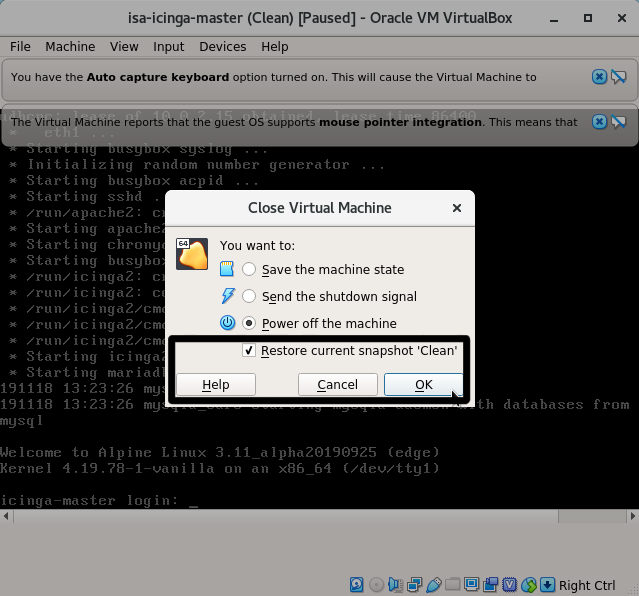
\includegraphics[width=0.67\linewidth]{files/vbox-shutdown.png}
	\label{fig:shutdown}
\end{figure}
